%%%%%%%%%%%%%%%%%%%%%%%%%%%%%%%%%%%%%%%%%%%%%%%%%%%%%%%%%%%%%%%





%%%%% CHOOSE PAGE LAYOUT
% The most common choices should be below.  You can also do other things, like replacing "a4paper" with "letterpaper", etc.

% This one will format for two-sided binding (ie left and right pages have mirror margins; blank pages inserted where needed):
\documentclass[a4paper,twoside]{lahcenthesis}
% This one will format for one-sided binding (ie left margin > right margin; no extra blank pages):
%\documentclass[a4paper]{lahcenthesis}
% This one will format for PDF output (ie equal margins, no extra blank pages):
%\documentclass[a4paper,nobind]{lahcenthesis} 



%%%%% SELECT YOUR DRAFT OPTIONS
% Three options going on here; use in any combination.  But remember to turn the first two off before
% generating a PDF to send to the printer!

% This adds a "DRAFT" footer to every normal page.  (The first page of each chapter is not a "normal" page.)
\fancyfoot[C]{\emph{DRAFT Printed on \today}}  

% This highlights (in blue) corrections marked with (for words) \mccorrect{blah} or (for whole
% paragraphs) \begin{mccorrection} . . . \end{mccorrection}.  This can be useful for sending a PDF of
% your corrected thesis to your examiners for review.  Turn it off, and the blue disappears.
\correctionstrue


%%%%% BIBLIOGRAPHY SETUP
% Note that your bibliography will require some tweaking depending on your department, preferred format, etc.
% The options included below are just very basic "sciencey" and "humanitiesey" options to get started.
% If you've not used LaTeX before, I recommend reading a little about biblatex/biber and getting started with it.
% If you're already a LaTeX pro and are used to natbib or something, modify as necessary.
% Either way, you'll have to choose and configure an appropriate bibliography format...

% The science-type option: numerical in-text citation with references in order of appearance.
\usepackage[style=numeric-comp, sorting=none, backend=biber, doi=false, isbn=false]{biblatex}

\usepackage{graphicx}
\usepackage{pdfpages}
\newcommand*{\bibtitle}{References}

% The humanities-type option: author-year in-text citation with an alphabetical works cited.
%\usepackage[style=authoryear, sorting=nyt, backend=biber, maxcitenames=2, useprefix, doi=false, isbn=false]{biblatex}
%\newcommand*{\bibtitle}{Works Cited}

% This makes the bibliography left-aligned (not 'justified') and slightly smaller font.
\renewcommand*{\bibfont}{\raggedright\small}

% Change this to the name of your .bib file (usually exported from a citation manager like Zotero or EndNote).
\addbibresource{references.bib}


% Uncomment this if you want equation numbers per section (2.3.12), instead of per chapter (2.18):
%\numberwithin{equation}{subsection}



%%%%% THESIS / TITLE PAGE INFORMATION
% Everybody needs to complete the following:
\title{Movie Review Generation}
\author{Thomas Palmer}
\college{Goldsmiths College}

% Master's candidates who require the alternate title page (with candidate number and word count)
% must also un-comment and complete the following three lines:
%\masterssubmissiontrue
%\candidateno{933516}
%\wordcount{28,815}

% Uncomment the following line if your degree also includes exams (eg most masters):
%\renewcommand{\submittedtext}{Submitted in partial completion of the}
% Your full degree name.  (But remember that DPhils aren't "in" anything.  They're just DPhils.)
\degree{B. Computer Science}
% Term and year of submission, or date if your board requires (eg most masters)
\degreedate{\today}


%%%%% YOUR OWN PERSONAL MACROS
% This is a good place to dump your own LaTeX macros as they come up.

% To make text superscripts shortcuts
	\renewcommand{\th}{\textsuperscript{th}} % ex: I won 4\th place
	\newcommand{\nd}{\textsuperscript{nd}}
	\renewcommand{\st}{\textsuperscript{st}}
	\newcommand{\rd}{\textsuperscript{rd}}



%%%%% THE ACTUAL DOCUMENT STARTS HERE
\begin{document}



%%%%% CHOOSE YOUR LINE SPACING HERE
% This is the official option.  Use it for your submission copy and library copy:
\setlength{\textbaselineskip}{22pt plus2pt}
% This is closer spacing (about 1.5-spaced) that you might prefer for your personal copies:
%\setlength{\textbaselineskip}{18pt plus2pt minus1pt}

% You can set the spacing here for the roman-numbered pages (acknowledgements, table of contents, etc.)
\setlength{\frontmatterbaselineskip}{17pt plus1pt minus1pt}

% Leave this line alone; it gets things started for the real document.
\setlength{\baselineskip}{\textbaselineskip}


%%%%% CHOOSE YOUR SECTION NUMBERING DEPTH HERE
% You have two choices.  First, how far down are sections numbered?  (Below that, they're named but
% don't get numbers.)  Second, what level of section appears in the table of contents?  These don't have
% to match: you can have numbered sections that don't show up in the ToC, or unnumbered sections that
% do.  Throughout, 0 = chapter; 1 = section; 2 = subsection; 3 = subsubsection, 4 = paragraph...

% The level that gets a number:
\setcounter{secnumdepth}{2}
% The level that shows up in the ToC:
\setcounter{tocdepth}{2}


%%%%% ABSTRACT SEPARATE
% This is used to create the separate, one-page abstract that you are required to hand into the Exam
% Schools.  You can comment it out to generate a PDF for printing or whatnot.
%\begin{abstractseparate}%
%	Your abstract text goes here.  
 % Create an abstract.tex file in the 'text' folder for your abstract.
%\end{abstractseparate}


% JEM: Pages are roman numbered from here, though page numbers are invisible until ToC.  This is in
% keeping with most typesetting conventions.
\begin{romanpages}

% Title page is created here
\maketitle

%%%%% DEDICATION -- If you'd like one, un-comment the following.
%\begin{dedication}
%This thesis is dedicated to\\
%someone\\
%for some special reason\\
%\end{dedication}

%%%%% ACKNOWLEDGEMENTS -- Nothing to do here except comment out if you don't want it.
\begin{acknowledgements}
 	\subsection*{Personal}

This is where you thank your advisor, colleagues, and family and friends.


\subsection*{Institutional}

If you want to separate out your thanks for your college or dept.
\end{acknowledgements}

%%%%% ABSTRACT -- Nothing to do here except comment out if you don't want it.
\begin{abstract}
	Your abstract text goes here.  

\end{abstract}

%%%%% MINI TABLES
% This lays the groundwork for per-chapter, mini tables of contents.  Comment the following line
% (and remove \minitoc from the chapter files) if you don't want this.  Un-comment either of the
% next two lines if you want a per-chapter list of figures or tables.
\dominitoc % include a mini table of contents
%\dominilof  % include a mini list of figures
%\dominilot  % include a mini list of tables

% This aligns the bottom of the text of each page.  It generally makes things look better.
\flushbottom

% This is where the whole-document ToC appears:
\tableofcontents

\listoffigures
	\mtcaddchapter
% \mtcaddchapter is needed when adding a non-chapter (but chapter-like) entity to avoid confusing minitoc

% Uncomment to generate a list of tables:
%\listoftables
%	\mtcaddchapter

%%%%% LIST OF ABBREVIATIONS
% This example includes a list of abbreviations.  Look at text/abbreviations.tex to see how that file is
% formatted.  The template can handle any kind of list though, so this might be a good place for a
% glossary, etc.
% First parameter can be changed eg to "Glossary" or something.
% Second parameter is the max length of bold terms.
\begin{mclistof}{List of Abbreviations}{3.2cm}

\item[NLG] Natural Language Generation - the field of research dedicated to the computational generation of natural sounding text.

\item[NLP] Natural Language Processing - the field of research dedicated to the understanding and processing of human language.



\end{mclistof} 


% The Roman pages, like the Roman Empire, must come to its inevitable close.
\end{romanpages}


%%%%% CHAPTERS
% Add or remove any chapters you'd like here, by file name (excluding '.tex'):
\flushbottom

%\begin{savequote}[8cm]
%\textlatin{Neque porro quisquam est qui dolorem ipsum quia dolor sit amet, consectetur, adipisci velit...}
%
%There is no one who loves pain itself, who seeks after it and wants to have it, simply because it is pain...
%  \qauthor{--- Cicero's \textit{de Finibus Bonorum et Malorum}}
%\end{savequote}

\chapter{\label{ch:1-intro}Introduction} 

\minitoc

\section{Overview of the System}
This project attempts to create believable reviews for a movie given a corpus of text (such as reviews of that specific film taken from users of IMdB) which discusses it. 

There are a collection of systems I have implemented for this project which range from simple to greater complexity, which attempt to create believable text in review or discursive form. \\

The first system is a review website created in PHP, using a MySQL database to host content, which host movie reviews generated as well as to be a platform for collecting user data, feedback and analytics. As well as this system - a further PHP website for comparative review testing has been created to supplement the gathering of feedback.\\

The second system is a bot for the website Twitter, which uses Markov chains to reply to tweets discussing movies and post discussion in the tags for specific films, in order to drive traffic towards the review website as well as explore the ability of Markov chains to generate believable text.\\

The next system is a collection of methods used in generating reviews for movies. The first being the use of a Markov Chain model on a corpus of movie review text. Next, which aims to be more insightful is a template-based system which mines sentiment from a corpus of text about a specific film as part of speech tagging to create text based on opinions expressed in the corpus of text given, and outputs a structured review. The third system attempts to use a Natural Language Generation methodology in creating a review, following the 5 part methodology proposed by Dale and Reiter.

\section{Motivation}

The Internet is a vast resource for opinion, thoughts and discourse on many topics such as film and other media. There are countless reviews, ratings and comments about any given topic, and this is a valuable resource to mine in order to extract opinion and detail about what is being discussed.\\

The applications of Natural Language Processing (NLP) and more specifically Natural Language Generation (NLG) are powerful in this domain.  Opinion mining and understanding of such a vast field of reviewers and people engaging in discussion can provide interesting data and context on the success of a film. Such methods are able to process and understand a very large corpus of text far faster than one may be able to read through all of the writings on a film manually. \\

This project aims to create a system that addresses these issues, and generates a review of a movie that is both coherent and insightful, related to the corpus of movie review text it is given. It would prefer to be somewhat summarative of the corpus it is given, but due to the natural polarity of movie review text it would be difficult to engineer and assess quite how summarative a piece of work may be.\\

A system of this kind could be employed in business - for example, reviews and articles about cinema can have a profound effect on their commercial success, and if enough respected reviewers pan a film it may become necessary to understand why - and a tool such as this could aid this process.\\

It could also be employed at a consumer level in order for a user to quickly evaluate whether or not they wanted to watch a film or buy a product based on a vast amount of review text that exists rather than the opinion of a singular reviewer.\\
As well as this, it may simply be used for entertainment purposes, to fool or generate conversation about a film in particular.\\

\section{Thesis Structure}
This thesis is structured as follows:\\
Chapter 2: This chapter provides background research into generating prose as well as evaluating text and a review of literature in these topics.\\ It also includes an exploration of past works in similar generative projects as well as human-like text agents such as Twitter bots.\\
Chapter 3: A specification of the project, including the design and implementation details of the systems discussed in this dissertation.\\
Chapter 5: Testing of the systems performed are documented in this chapter.\\
Chapter 6: An evaluation of the systems created.\\
Chapter 7: A conclusion, discussing the outcomes of the systems implemented.\\
After this, a bibliography and appendices section are included.


%\begin{savequote}[8cm]
%Alles Gescheite ist schon gedacht worden.\\
%Man muss nur versuchen, es noch einmal zu denken.
%
%All intelligent thoughts have already been thought;\\
%what is necessary is only to try to think them again.
%  \qauthor{--- Johann Wolfgang von Goethe \cite{von_goethe_wilhelm_1829}}
%\end{savequote}

\chapter{\label{ch:2-litreview}Background}

%\minitoc

\section{Introduction}

This document introduction won't serve as a complete primer on \LaTeX.  There are plenty of those online, and googling your questions will often get you answers, especially from \url{http://tex.stackexchange.com}.

Instead, let's talk a little about a few of the features and packages lumped into this template situation.  The \verb|savequote| environment at the beginning of chapters can add some wittiness to your thesis.  If you don't like the quotes, just remove that block.

For when it comes time to do corrections, there are two useful commands here.  First, the \verb|mccorrect| command allows you to highlight a short correction \mccorrect{like this one}.  When the thesis is typeset normally, the correction will just appear as part of the text.  However, when you declare \verb|\correctionstrue| in the main \verb|Oxford_Thesis.tex| file, that correction will be highlighted in blue.  That might be useful for submitting a post-viva, corrected copy to your examiners so they can quickly verify you've completed the task.

\begin{mccorrection}
For larger chunks, like this paragraph or indeed entire figures, you can use the \verb|mccorrection| environment.  This environment highlights paragraph-sized and larger blocks with the same blue colour.
\end{mccorrection}

Read through the \verb|final-report.tex| file to see the various options for one- and two-sided printing, including or excluding the separate abstract page, and turning corrections and draft footer on or off, and the separate option to centre your text on the page (for PDF submission) or offset it (for binding).  There is also a separate option for master's degree submissions, which changes identifying information to candidate number and includes a word count.  (Unfortunately, \LaTeX has a hard time doing word counts automatically, so you'll have to enter the count manually if you require this.)

\section{Fraud Detection}
\label{app:fraud}

Within months of Röntgen's discovery of the X-ray in \mccorrect{1895}\cite{gagliardi_rontgen_1996}, cardiac pathology was being investigated via non-invasive imaging \cite{gagliardi_cardiac_1996}.  Over the intervening years, cardiac imaging modalities and techniques have advanced significantly.  Clinically, cardiac imaging is used for two broad purposes: diagnosis of pathophysiology and guidance of interventional procedures.  These applications impose different requirements on imaging equipment, image acquisition time, computational complexity, spatial and temporal resolution, and tissue discrimination.  The common diagnostic and interventional cardiac imaging techniques in current clinical practice are reviewed below.  An accessible introduction to the physics of medical imaging can be found in Webb's \textit{Introduction to Biomedical Imaging} \cite{webb_introduction_2002}.  A comprehensive overview of the use of imaging in clinical cardiology is presented in Leeson's \textit{Cardiovascular Imaging} \cite{leeson_cardiovascular_2011}.

\subsection{Machine Learning}
\label{sub:machine-learning}

Beyond the chest X-ray (`plain film'), the key non-invasive imaging modalities in diagnostic cardiology are echocardiography, magnetic resonance imaging, and X-ray computed tomography, which are reviewed below.  Nuclear medicine, including positron emission tomography (PET) and single-photon emission computed tomography (SPECT), are not discussed here, as they do not play a role in the chapters to follow.

\subsubsection{Recurrent Neural Network}
Most all previous RNN based~\emph{dst~forecasting}
research~\cite{pallocchia:2006} has relied on
batch\footnote{batch refers to models trained on an in sample data
set and then evaluated on an out of sample data set in which no
learning occurs in the out of sample data set.} algorithms for
training the RNN. Batch training algorithms are unable to
incorporate newly arrived information into the model parameters
without re-processing the entire data set (which is a costly
operation). Furthermore, the training algorithms used thus far for
training the RNNs on~\emph{dst~forecasting} (all of which have been batch
first order gradient descent) are known to be susceptible to local
minima, and uncertain convergence. This has been a bottleneck in the
area (and may stifle future progress in neural based forecasting of
geomagnetic phenomena), as well performing models are difficult to
obtain, and new events can not readily be incorporated into the
model for improved forecasts.


\begin{figure}
\centering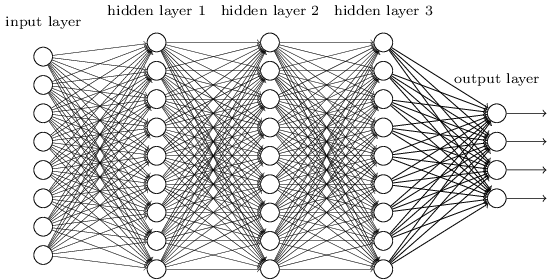
\includegraphics[width=0.7\textwidth]{figures/rnn.png} 
\caption[A schematic representation of the fully recurrent neural
network architecture.]{A schematic representation of the fully recurrent neural
network architecture}
\label{fig:fourchamber}\end{figure}


\subsubsection{Rand Index Algorithm}

%\begin{figure}
%\centering\includegraphics[width=0.7\textwidth]{figures/sample/Gray498.png} 
%\caption[Four-chamber illustration of the human heart.]{Four-chamber illustration of the human heart.  Clockwise from upper-left: right atrium, left atrium, left ventricle, right ventricle.}
%\label{fig:fourchamber}\end{figure}







The use of acoustic waves for medical diagnosis, inspired by naval sonar, was initially developed in the 1940s \cite{gagliardi_ultrasonography_1996}.  By 1954, the first clinically useful cardiac ultrasound -- examining motion of the mitral valve in stenosis -- was reported \cite{edler_ultrasonic_1957}.  These early scans were one-dimensional images (`A-mode'), sometimes repeated to generate a time axis (`M-mode').   The sector-scanning probe was developed in the 1970s \cite{bom_ultrasonic_1971,griffith_sector_1974}, leading to the `B-mode' that a modern cardiologist would recognise as an echocardiogram.



\chapter{\label{ch:3-design} Design}

%\minitoc

\section{Introduction}

\section{Aims and Objectives}
\subsection{Aims}

The primary aim of this project is to explore methods for text generation and then develop a system through which prose about movies can be generated. This prose should be in the form of a movie review, and should pick the most recurrent points or themes in a corpus of movie reviews discussing a singular movie.

\subsection{Objectives}

To develop a natural language generation system which picks points from multiple review texts and uses them to structure an informed review.\\
To develop an online platform to host generated movie reviews which can gather feedback and data on the reception of said review.\\
To develop an autonomous bot that can discuss movies (or at least reply with an opinion of a movie) over twitter. Ideally this would drive traffic towards the movie review blog which hosts reviews made by the bot.

\section{Movie Review Generation}

\subsection{Markov Chain for Text Generation}
\subsection{Template-Based System for Text Generation}
The design of this system started with the premise of filling out template sentences for segments of a review in a random fashion until a text of a satisfactory size is produced. The initial idea being that an introduction is filled in, then a brief plot synopsis, some text evaluating the performances of actors and noteworthy crew (such as the director or writers) and then a closing statement regarding whether or not its worth seeing a film.\\

The first step of the template system is data gathering.

It web scrapes a corpus of movie reviews for a given movie from IMdB. These are user reviews taken from a movie's reviews page, and an amount are taken sorted by their highest rating. Then it web scrapes plot synopsis, also from IMdB this is then summarized using the TextRank algorithm. It finally uses themoviedb's API to gather metadata about a film, such as cast crew and genre.\\


The second step in this process is then forming an understanding of that data.
First is the separation each review text into a large list of sentences so that they can be tagged and analyzed for sentiment.
Categorise each sentence as about a particular topic or person (cast, crew, director), using the metadata gathered from the OMdB API to match sentences to these topics.\\

The final step is then filling in the reviews templates until completion.
Builds an introduction based on a template, a plot summary after that, a body of review text, and then a closing statement based on the template.
Templates are filled with words determined by sentiment, and adjectives and adverbs mined from part of speech tagging sentences regarding the topic discussed in the template sentence.\\


\subsection{NLG System}

\section{Twitter Bot}
The Twitter bot exists in order to drive traffic towards the reviews generated and also act as a test of generating text in shorter formats than review - for example the markov chains discussed earlier are much more believable if you don't let them go on for too long. The limit of 144 characters is certainly suitable for this.\\
The bot itself uses a twitter API wrapper called Tweepy, which handles Twitter API requests required in order to make posts, search and navigate twitter.\\
There are a number of behaviours programmed for the bot to gather attention and direct users towards the website. The first is simply the automated posting of links to movie reviews generated, with a template message that reads along the lines of "Read my review for #filmname here".\\
The next behaviour is replying to posts which have been identified to be about the movie in question with comments generated from a markov chain of other tweets about the movie.\\ 


\section{Blog Website}
The design of the blog website is relatively simple. It is a Wordpress-like blogging website written in PHP, wish a MySQL database that stores the reviews, user information and the comments made and analytics for the site.\\
I have chosen MySQL and PHP as they are languages I am familiar with, and have worked using before, as well as their being suitable for the task of a small blogging platform.\\
The website itself is a front-page which lists paginated results for movie reviews written by the movie review generator, an interface for making/creating posts, and a way to view the reviews in full. It also has user comments for gathering qualitative feedback and page visits and engagements are tracked using Google analytics and a MySQL hit-counter.\\




\chapter{\label{ch:5-testing} Testing}

%\minitoc

\section{Introduction}
Testing each part of this system involves checking primarily that outputs are what they should be (or at least as expected due to the outputs being semi-random in places), as we are handling a lot of data which is scraped from the internet, using APIs and other tools for gathering data from the internet. 


\section{Markov Chain System}
\subsection{Testing}
This involved simply testing that the program executed at the correct point and could handle both of the input sources I gave it, as well as that the Markov table is built successfully from the two types of input and the actual obtaining of these inputs also works.

\begin{center}
	\begin{tabular}{||m{15em} m{10em} m{10em} m{4em}||} 
		
		\hline
		Test Case & Expected & Actual & Status \\ [0.5ex] 
		\hline\hline
		Twitter corpora obtained& Twitter API returns search data& Twitter API returns search data& Pass\\
		\hline
		Twitter corpora parsing& All non-reply data is trimmed, only tweet text remains& URLS of images are still retained& Fail\\
		\hline
		Markov Table Building - Single text source& Table builds successfully& Table builds successfully& Pass\\
		\hline
		Markov Table Building - Twitter as Text source& Table builds successfully & Table builds successfully& Pass\\
		\hline
		Text Generates from single review input& Text is output, no runtime error& output obtained& pass\\
		\hline
		Text generates from Twitter search corpora& Text is output, no runtime error& output obtained& pass\\ [1ex] 
		\hline
	\end{tabular}
\end{center}

\subsection{Summary of Changes Made}
Images and URLS are still retained when the text is parsed so I introduced a check for hyperlinks and removed those from the text as well, since the reuse of this images and urls is not something I necessarily want.

\section{Template System}
\subsection{Testing}
\begin{center}
	\begin{tabular}{||m{15em} m{10em} m{10em} m{4em}||} 
		\hline
		Test Case & Expected & Actual & Status \\ [0.5ex] 
		\hline\hline
		IMDB Corpora Scraped& n*10 reviews scraped& n pages of reviews are scraped for a particular review& pass\\
		\hline 
		IMDB Plot Summary Scraped& A plot-summary is scraped from IMdB& Plot summary scraped successfully& pass\\
		\hline
		Metadata obtained from API& Cast, Director, Crew, Genre all scraped from TMdB & The aforementioned data is all obtained& pass\\
		\hline
		Cast and Crew sentiment assignation& Cast, crew, director sent all assigned appropriately &Odd repetition and multiple of the same text to one cast member, some members not mentioned and assigned to a sentence anyway & Fail\\
		\hline
		Adverbs and adjectives searching&An adverb or adjective is obtained from a given corpora& Either adverb or adjective is returned, unless there aren't any one available& fail\\
		\hline
		Intro templates fulfil successfully&Each pre-defined introduction section is fulfilled when asked& They all were filled succesfully& Pass\\
		\hline
		Main body templates fulfil successfully&Each pre-defined introduction section is fulfilled when asked& They all were filled succesfully& Pass\\
		\hline
		Outro templates fulfil successfully&Each pre-defined introduction section is fulfilled when asked& They all were filled succesfully& Pass\\
		\hline
		Full review text&A full review text is obtained& Full review text is indeed obtained& Pass\\ [1ex] 
		\hline
	\end{tabular}
\end{center}

\subsection{Changes Made}
Cast and crew being assigned individually tagged sentences that mentioned them was broken in a number of ways. For one, it would search for instances of either  name of a cast or crew member by spitting the name obtained from the API into a list based on where spaces occur in that name or their role. This meant that people with roles such as "The man with the hat" would be overly represented in the sample due to "The" and other common words being in their name. I included a list of names that could be removed from these acceptable names in order to mitigate this.\\
As well as this, the cast and crew members were being multiplied as it was not correctly identifying when cast and crew members had already had sentences assigned to them, so kept creating instances for them in the list. Instead of a list of actor/cast names, accompanied by a nested list of sentences that mention them with their sentiment polarity, it would mention the actor and cast member every single time, creating a much larger and much less efficient list. This was fixed so the data collection worked as intended.\\
In cases where adverbs or adjectives weren't present in the corpora provided, there was no method for handling this sentiment request. This was changed so that at the very least a basic adjective or adverb would be returned in the stead of something more interesting. "Good" or "well" would be returned in these cases, which is at least going to fulfil the template.



\section{NLG System}
\subsection{Testing}
Primarily involves testing that the new data obtained works as intended, as well as each stage in the NLG process was producing a correct result that could lead to an output.
\begin{center}
	\begin{tabular}{||m{15em} m{10em} m{10em} m{4em}||} 
		\hline
		Test Case & Expected & Actual & Status \\ [0.5ex] 
		\hline\hline
		Past Work Mining&&&\\
		\hline
		Most Important Cast/Crew&&&\\ 
		\hline
		Intro Structure&&&\\
		\hline
		Body Structure&&&\\
		\hline
		Outro Structure&&&\\
		\hline
		Intro aggregation&&&\\
		\hline
		Body aggregation&&&\\
		\hline
		Outro Aggregation&&&\\
		\hline
		Intro lexchoice&&&\\
		\hline
		Body lexchoice&&&\\
		\hline
		Outro lexchoice&&&\\
		\hline
		Referring Expressions&&&\\
		\hline
		Realisation&&&\\
		\hline	
		Full text& A full text is obtained, from start to beginning& We get a full review& Pass\\ [1ex] 
		\hline
		
	\end{tabular}
\end{center}

\subsection{Changes Made}



\section{Website Testing}
\subsection{Testing of Blog Website}
This testing mainly involved testing that aspects of the system that face the users work, as the rest can be handled by the PHPMyAdmin portal for interfacing with the database.
\begin{center}
	\begin{tabular}{||m{15em} m{10em} m{10em} m{4em}||} 
		\hline
		Test Case & Expected & Actual & Status \\ [0.5ex] 
		\hline\hline
		Create Account Submit& Account submits, database updates, pwd hashes+salts& pwd hash+salt successful& pass\\
		\hline
		Login Submit (correct details)&Login is successful&Login is successful& pass\\
		\hline
		Login Submit (incorrect details)&Login is unsuccessful&Login is unsuccessful& pass\\
		\hline
		Log Out Clicked&Account is logged out&Account is logged out&pass\\
		\hline
		Review Submit&Details are submitted into the db&Review is submitted successfully& pass\\
		\hline
		Review Edit Submit&Review is updated in database&Review is updated& Pass\\
		\hline
		Main Page Loads&Paginated data loads, review loads chronologically&Reviews load& Pass\\
		\hline
		Individual Review Loads&Review loads, comments section loads& Review and comments section load& Pass\\
		\hline
		Comments Submit&Comments insert into database for correct entry&Comments insert correctly&Pass\\
		\hline
		Comments Load&Comments load for correct entry& Comments do load& Pass\\ [1ex]
		\hline
	\end{tabular}
\end{center}


\subsection{Testing of Turing-Like Test Website}
Primarily involved checking data entry worked completely.

\begin{center}
	\begin{tabular}{||m{15em} m{10em} m{10em} m{4em}||} 
		\hline
		Test Case & Expected & Actual & Status \\ [0.5ex] 
		\hline\hline
		Data Fetches& Data for each review loads& It does& Pass\\
		\hline
		Completion of First Item&SQL executes successfully, update visible on database& Update is successful& Pass\\
		\hline
		Completion of Last Item&SQL executes successfully, visible on db& Update is successful& Pass\\ [1ex] 
		\hline
	\end{tabular}
\end{center}

\section{Twitter Bot}
\subsection{Testing of Twitter Bot}
I have mostly decided to test that the Bot runs as expected, although it only has two outputs.
\begin{center}
	\begin{tabular}{||m{15em} m{10em} m{10em} m{4em}||} 
		\hline
		Test Case & Expected & Actual & Status \\ [0.5ex] 
		\hline\hline
		Generating Promotional Tweet& Posts & Post Successfully & Pass \\ 
		\hline
		Gen promo tweet (length intentionally too long) & Doesn't post, code continues to execute & As prior& Pass\\
		\hline
		Generate Markov Tweet (Acceptable Length) & Posts & Tweet outside of character limit (far too often to be inadmissable) & fail\\
		\hline
		Gen Markov tweet (length intentionally too long) & Doesn't post, code continues to execute & As prior& Pass\\ [1ex] 
		\hline
	\end{tabular}
\end{center}

\subsection{Changes Made}
First, the bot would far more often than not attempt to create tweets that were too long to be postable using the Markov model, as it would not check for a character limit to have been exceeded due to this not being needed when simply generating Markov text. I added a parameter to check that things would work. \\
Then without my noticing, the bot would post tweets that were a single word long due to a mistake checking the tweets were less than the character limit and breaking the chain. It checked that the tweet was longer than 144 characters as a conditional for continuing, which no entry was as it was a single word to begin with, and just returned that first input.\\


\chapter{\label{ch:6-evaluation} Evaluation}

%\minitoc

\section{Introduction}
A well documented issue with Natural Language Generation and other methods for generating prose is the problems with evaluating such systems. It can be hard to extract statistical data about how natural or believable the language sounds as well to derive performance measures for such a system in a way you could with other systems such as machine learning algorithms with more obvious relevant performance measures such as time and space complexity and measures of accuracy. These are not particularly useful in the case of a NLG system where an output being created in a reasonable amount of time is sufficient.\\

The majority of my evaluation was planned to be on the review of comments and replies observed on twitter and the blogging website, and a separate scenario where the believability of review generated is asked for in a test environment against real movie reviews gathered from the internet.

\section{Markov Chain text generation}
This was used as my baseline for generating movie prose, although it definitely served to be the least feasible of all the methods used. This was because the chains mostly produced complete nonsense when the corpora was expanded or the number of words represented as a node in a chain were decreased.\\
From my own observations, the text generated seemed more likely to be coherent at larger numbers of words per point in the chain, but were much more likely to form linear chains and copy text from the corpora verbatim, instead of producing something new. Smaller word counts would produce more original texts but would lose coherence much more quickly and fall apart much more quickly over larger output texts.
(FIGURE HERE)

\section{Engagement With Twitter Bot}
The Twitter bot produced posts generated from Markov chains formed from corpora of tweets produced from twitter searches for terms related to certain movies. Every other tweet attempted to promote the blog website's hosted reviews.

\subsection{Results}
While the bot was running between the 17th of April to the 11th of May - a 25 day period - the tweets made generated a total of 13500 impressions. An impression is defined as any time a user has seen a tweet on Twitter.\\
An average of 551 impressions per day has been achieved while the bot has been running, although this has not amounted to a great amount of qualitative data - which is what I had hoped to obtain. The Twitter bot received very little attention in terms of link-clicks, follows and likes, even with hash tags for popular or controversial movies being used. A total of 34 link-clicks were obtained over this period, which is a very small amount relative to the number of overall engagements or impressions made over the time period. There were no real interactions with the bot outside of being followed by 3 other automated twitter accounts, all but one of which has since unfollowed. Occasionally words would trigger other bots to retweet them, but no human-controlled interactions were observed. \\
(FIGURE OF TWITTER ANALYTICS DATA)

\subsection{Observations}
The Twitter bot did not directly interact with any twitter users other than making posts, which may have limited the effect of its outreach. It would be interesting to implement post-liking or replying behaviours in the bot at a later date and see if that has an increased impact on the attention it receives. As well as this, the URL of the blog website may have been offputting towards potential readers and could have had an impact on the number of link clicks I have observed.\\
I would not say the bot was greatly successful in generating attention for the review website, due to the low number of link clicks had, but it did attract a small amount of attention using these relatively simple generative techniques.


\section{Comments and Interaction with Blog Website}
A number of reviews generated through the template system were hosted on the blog website, in order to see if they would receive any replies or feedback at all. This was later expanded to include reviews from the NLG system as well once that was implemented. It consists of an index page which loads a paginated list of movie reviews with a shortened preview of the article written with a link to the full text. The full text displays with a comments section below it.

\subsection{Results}
Unfortunately, there were no comments were left on the blog website, which is a shame as it would have been an interesting measurement of the believability of the reviews. Google analytics has however observed 53 unique sessions over the month the bot was active, involving 39 users generating 123 pageviews. The average number of pages visited in a session is 2.32 which indicates that users will have attempted to read at least one review, and clicked on to the homepage to view the rest of the site. The average session duration was 57 seconds, which indicates that at least some of the users stuck around long enough to attempt to read a review, although not all of them will have.\\

(FIGURE OF GOOGLE ANALYTICS DATA)
\subsection{Observations}
I believe that a small, but not great amount of success was had from the Twitter bot generating this many unique sessions, although a failure of the content to be engaging enough to generate comment and feedback.\\
It is a valid criticism that the hosting of the website on the Department of Computing servers could throw people off from following the link and interacting with the website, as it is not a tidy URL (doc.gold.ac.uk/~tpalm003/reviews/index.php vs. something like tomsreviews.com) with an easily recognisable domain.\\
Another criticism is that the design of the blog is fairly simplistic and that its design may not be as convincing as other blog platforms for hosting movie reviews because of this.\\


\section{Turing Test Scenario}
In order to collect more detailed feedback on the NLG system, I set up a Turing-like test. Users were shown sentences and full reviews which were generated via the NLG system implemented, as well as real sentences and full reviews written by IMdB users. These were ordered randomly, and 4 examples of each case were selected. The users were shown these in a randomized order so there were no contextual clues as to whether or not the review was human or not, although the order that each user is shown the data was the same.

\subsection{Results}
I was able to obtain a good amount of feedback on the NLG system through this system. 11 respondents participated in the test (and 9 provided feedback for each of the examples given) and I managed to obtain interesting data on how the NLG system performs on the sentence and full text levels.\\
Generally, people found the full review texts that were generated to be less coherent and less human-like than real reviews, although the first review they were shown that was generated was received as coherent by 7 of the 11 respondents, and believably written by a human by 5, this effect wore off as they were shown more reviews and their structure was noticed. The final generated review seen was only thought to be human by 2 of the respondents, although voted coherent by 5 of 9 who made it to the end of the feedback session. \\

One user wrote "after you've read a couple of these the pattern becomes very obviously robotic," which demonstrates the point that the text generated follows a structure that is easy to recognise over multiple examples.\\

On the sentence level, it became very hard for participants to tell the difference between a generated sentence and a sentence taken from a real review, where the difference in scores closed, although some users were able to tell a sentence was generated due to it's pattern being seen in previous examples of full reviews. Generated sentences generally scored 8 out of 11 for how human they were each time, and between 5 and 7 out of 11 for their coherence. In contrast, real sentences scored between 5 and 8 out of 11 for how human they appeared, and 2 and 8 for how coherent they were. It is worth mentioning that I intentionally included sentences from less well written reviews in order to throw users off in terms of the exact way in which the reviews and sentences are generated by my system.\\



\subsection{Observations}
At the sentence level, it was difficult for readers to identify between the NLG system and real written reviews. However, this fell apart at the full review level when the initial review they read often failed to appear human-like and after more generated reviews were shown to them they also often became able to identify their structure and easily tell that they were generated through this.\\

The generation of sentences which convey sentiment and opinion seems to have gone well with the NLG system, where users struggle to tell them apart from real sentences. There is an issue with the variety of these sentences produced as some of the patterns and their handling are hard-coded and have flavour added to them from templates, as the data needed to form the actual opinion proved too difficult for me to extract.\\

It would appear that a weakness of the NLG system is the rigid document structuring that has been implemented, which seems to quite heavily impact the detection of these reviews over multiple documents. While this is less of a problem for single documents, it is certainly a worthwhile improvement to have more fluid and variable structures when generating documents to give the impression of a human author.\\
As well as this, another shortcoming of the NLG system is that to discuss a topic, data needs to be gathered on it to begin with. This is difficult in the case of discussing themes, plot synopses, tone and other higher concept topics that are discussed in reviews of art. An interesting area of improvement would be to implement some method for identifying and extracting data on some of these higher concepts from the review text corpora.




\chapter{\label{ch:7-conclusion} Conclusion and Future Work}

%\minitoc


\section{Review of Aims and Objectives}
I would say that this project has been moderately successful. Some feasible movie review text has indeed been generated, although not a lot and not in quite as large quantity or variety as I had aimed.
\subsection{Aims}
The aim of this project was to generate movie review prose that passed as human. This has been partially achieved, at the sentence level, although a movie review generated by any of my systems is not likely to pass as human, mostly due to the falling-apart of coherence outside of reporting facts and sentiments. I would not say this was achieved with great success, as little interaction with any of the systems aiming to pass as human has occurred.
\subsection{Objectives}
To explore methods for generating text which reviews film.\\
This object has certainly been met. I have explored a number of options for generating prose and implemented several methods for generating prose. I have looked at Markov models, Feed-Forward Neural Networks, Template based systems using context-free grammars, and Natural Language Generation architectures for generating prose.\\

To develop a natural language generation system which picks points from multiple review texts and uses them to structure an informed review.\\
Although I have implemented a system to meet his goal, the outputs generated do not manage to pass as human, and therefore I would not say I have met this objective with great success. As well as this, I made the concession of including templates into the NLG system in an attempt at making the system more human-like. More time to work on this system and I feel I could have met this objective more, although it would be partially template-based rather than strictly NLG.\\
To develop an online platform to host generated movie reviews which can gather feedback and data on the reception of said review.\\
I have met this objective successfully, although it had not been used as much as I had hoped for the collection of data. I could have put more time into the development of the site in order to make it more welcoming as well as hosting it on a URL that is potentially less scary than the URL of my system. (doc.gold.ac.uk/~tpalm003/reviews/index.php).\\
To develop an autonomous bot that can discuss movies (or at least reply with an opinion of a movie) over twitter. Ideally this would drive traffic towards the movie review blog which hosts reviews made by the bot.\\
This goal has been met, although its outreach is limited by the behaviours it puts into place. It makes posts and can post with hash-tags in an attempt to reach an audience, but it does not engage with twitter users through other interactions which would arguably make it a more believable bot, and at the very least have it seen by more people.\\


\section{Lessons Learned}
I have learned a number of things from this project, and had I started it again have a number of things I would do differently.
At the programming level, I've learnt a lot about using APIs as well as interracting with XML and JSON objects, as well as parsing text and working around very error-prone systems such as requesting data that might not necessarily exist.\\
I have had to research language processing and sentiment tagging, although I did opt to use libraries for these in my implementation as there was little point reimplementing code for systems with so many interacting elements.\\
I'd also not recommend relying on user data for systems that require finding attention in the real world (rather than appealing to users for feedback), as this has proven to be difficult to manage. As well as this I would recommend that people choose less subjective topics to implement NLG systems for if they were to choose NLG as a dissertation topic.


\section{Future Work}


\subsection{Improvements to current work}
An interesting area to explore is expanding the Twitter bot to handle behaviours other than self promotion and Markov chain generated text to reply to others. This would enable a system which intended to draw more attention to itself to operate in a more human-like manner as a real twitter user is more likely to utilize all of the features of the website and have a greater outreach through the use of replies - as notifications are sent directly to the user rather than having to search for a tweet generated by the bot.\\


It would also be interesting to expand the NLG system to handle a larger range of topics within movie generation for a more believable and comprehensive review of the film, and expand the grammars used to generate the sentiment-driven sentences. This would mostly include much more specific sentiment analysis using lists of sentiment tagged words for specific topics and themes that occur in cinema.\\

A further interesting expansion would be to target reviews at different audiences where people actively read for them, such as Youtube comments, reviews for Amazon streaming videos, and other websites that host users movie watchlists and reivews such as IMdB and letterboxd, as they have active communities that use will read these reviews to gage whether or not they want to watch a film, or for other purposes such as validating their own opinions. 

\section{The Future of Generative Film Reviews}
It is definitely safe to assume that the human-written review will not be made obsolete by reviews created from NLG methods for a long while yet. Given that a system like this would need to build its knowledge from some agent with enough insight to identify talking points and provide sentiment for each of these talking points, it is safe to say that without brilliant leaps in computer vision and audio processing, an article penned by a trusted reviewer is not going to be made redundant any time soon.









%% APPENDICES %% 
% Starts lettered appendices, adds a heading in table of contents, and adds a
%    page that just says "Appendices" to signal the end of your main text.
\startappendices
% Add or remove any appendices you'd like here:




\chapter{Evaluation Data}
\subsection{Twitter Analytics Data}



\centering
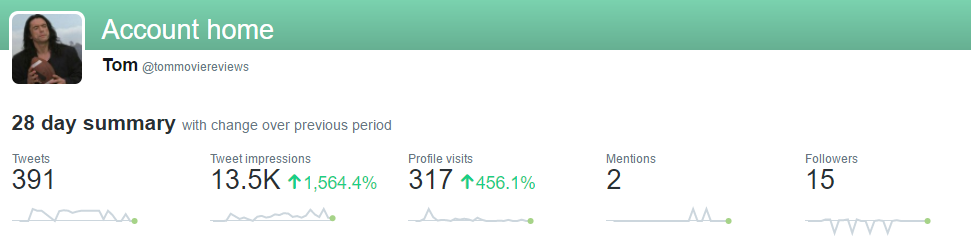
\includegraphics[width=0.7\linewidth]{figures/twitter_analytics/28daysummary}
%\caption{28 Day Summary of Twitter Bot Analytics}
\label{fig:28daysummary}


\centering
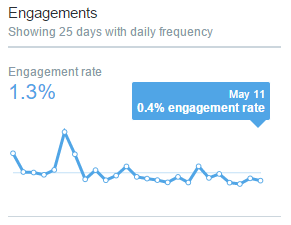
\includegraphics[width=0.7\linewidth]{figures/twitter_analytics/engagements}
%\caption{Total number of 'engagements' with twitter bot over active period}
\label{fig:engagements}


\centering
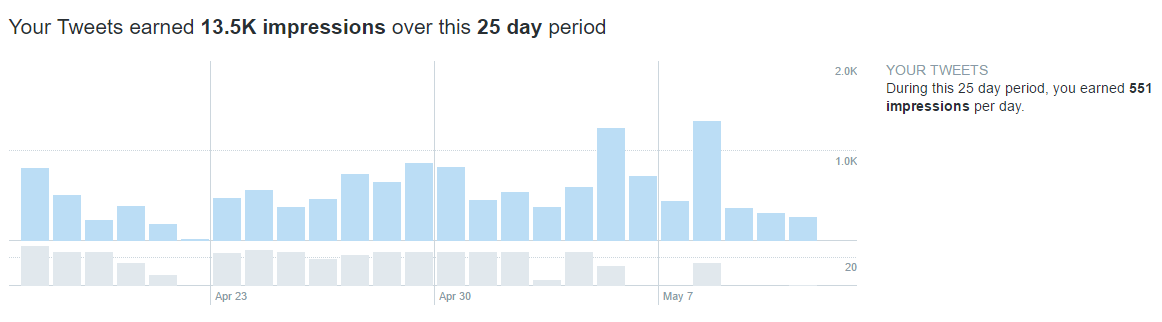
\includegraphics[width=0.7\linewidth]{figures/twitter_analytics/impressions}
%\caption{Total number of 'impressions' made by twitter bot over active period}
\label{fig:impressions}


\centering
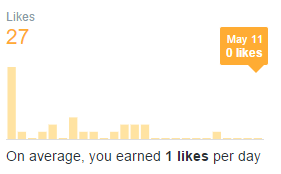
\includegraphics[width=0.7\linewidth]{figures/twitter_analytics/likes}
%\caption{Likes obtained over active period}
\label{fig:likes}

\centering
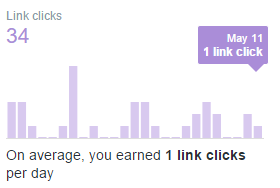
\includegraphics[width=0.7\linewidth]{figures/twitter_analytics/linkclicks}
%\caption{Links clicked over active period}
\label{fig:linkclicks}

\centering
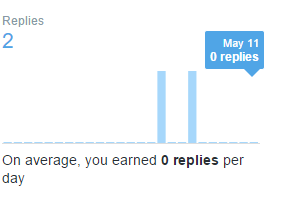
\includegraphics[width=0.7\linewidth]{figures/twitter_analytics/replies}
%\caption{Replies to posts made by bot over active period}
\label{fig:replies}

\centering
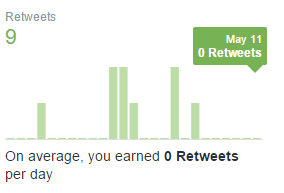
\includegraphics[width=0.7\linewidth]{figures/twitter_analytics/retweets}
%\caption{Retweets of posts made by bot over active period}
\label{fig:retweets}




\subsection{Google Analytics Data}

\centering
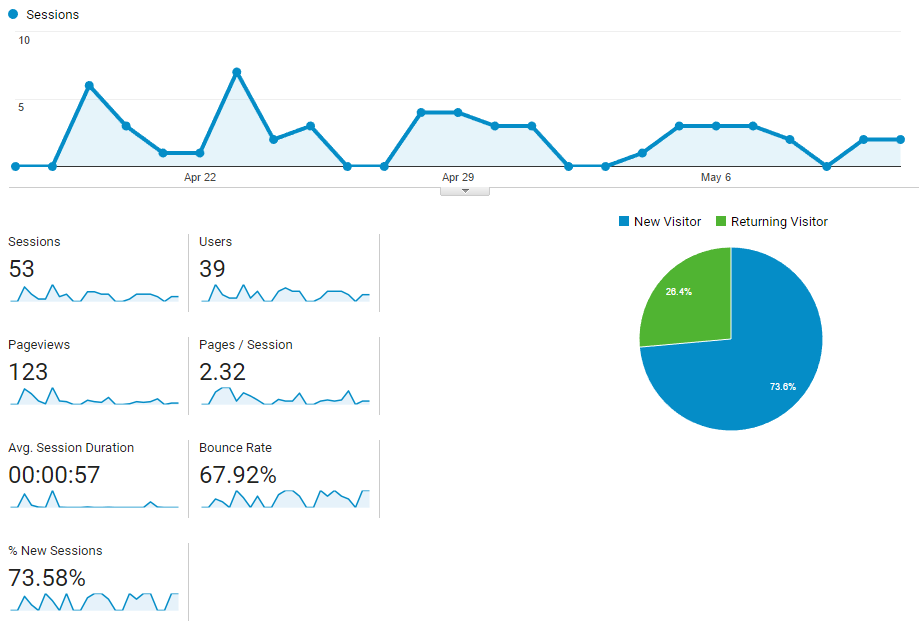
\includegraphics[width=0.7\linewidth]{figures/google_analytics/uniqueSessions}
%\caption{Google Analytics Screenshot showing unique sessions over test period}
\label{fig:uniquesessions}

\centering
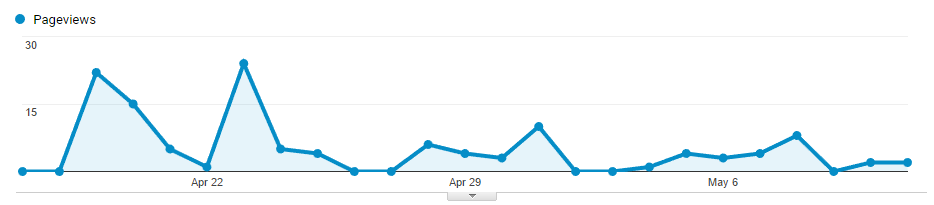
\includegraphics[width=0.7\linewidth]{figures/google_analytics/pageviews}
%\caption{Google Analytics Screenshot showing pageviews over test period}
\label{fig:pageviews}

\centering
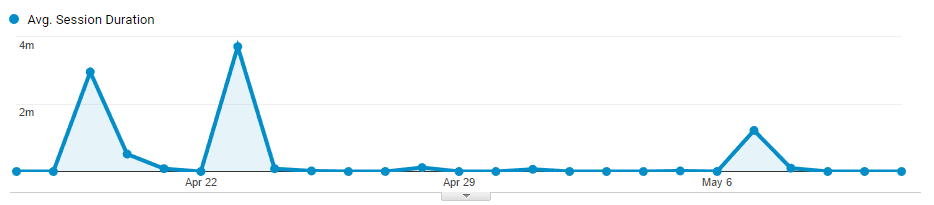
\includegraphics[width=0.7\linewidth]{figures/google_analytics/sessionDuration}
%\caption{Google Analytics Screenshot showing average session duration over test period}
\label{fig:sessionduration}

\chapter{Turing-Like Test Results}


\includepdf[pages={1-},scale=1]{"figures/turinglike_results/Review Feedback - reviewExcerpt (1)"}      


\chapter{Preliminary Project Report}


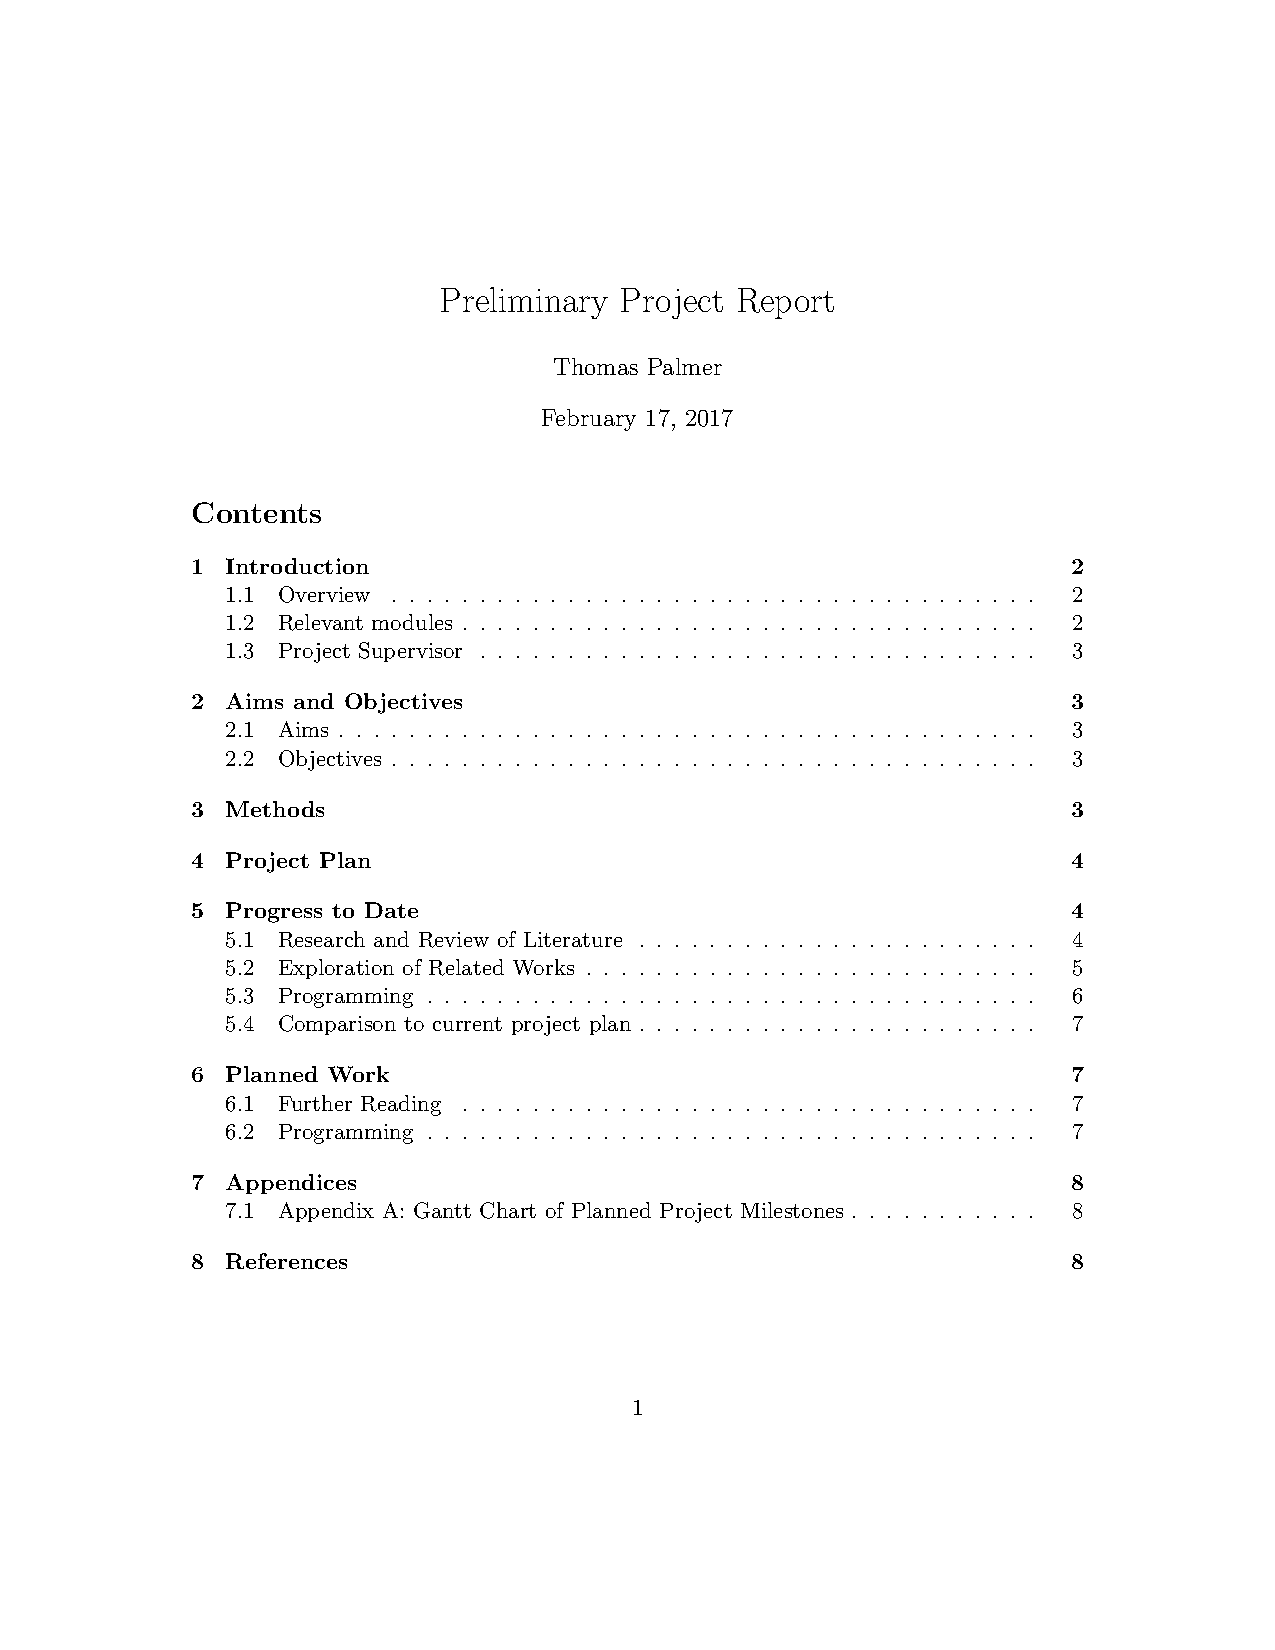
\includepdf[pages={1-},scale=1]{figures/preliminaryReport2}



\chapter{Project Logs}
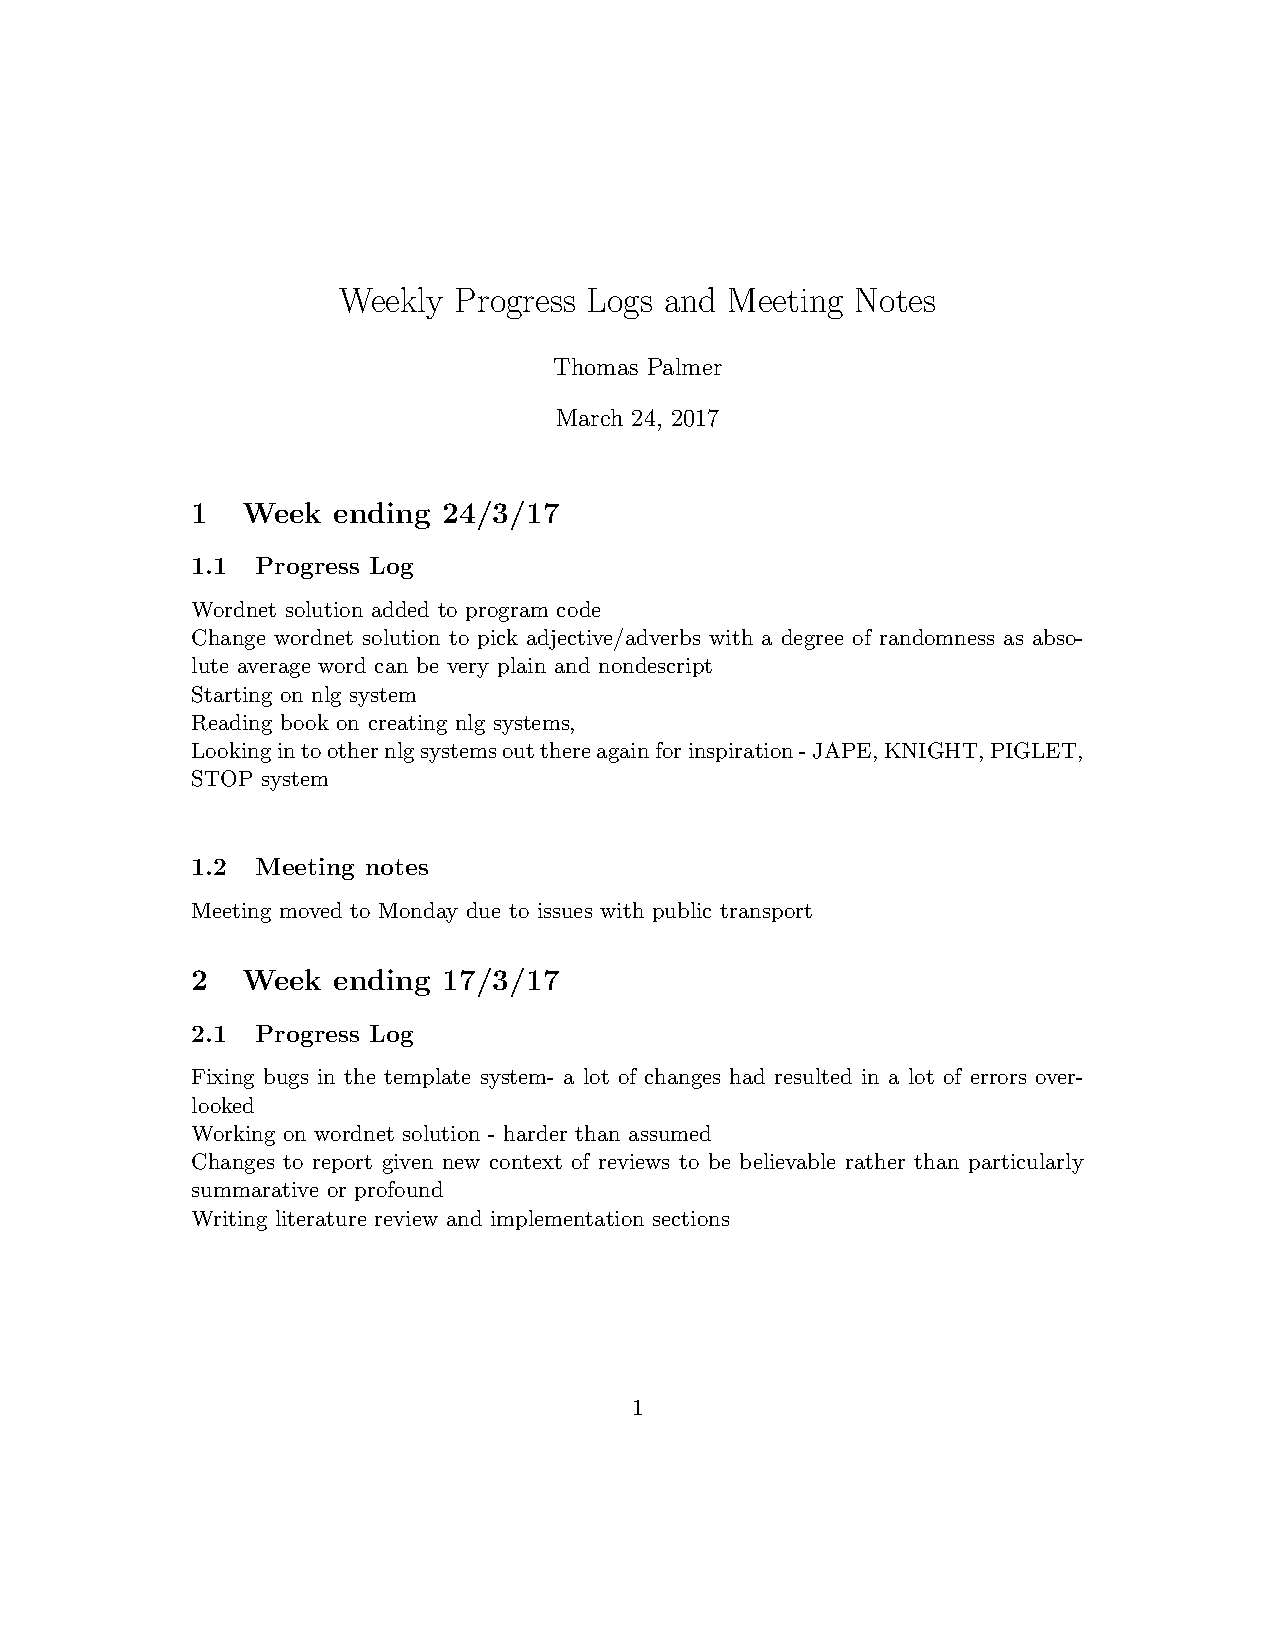
\includepdf[pages={1-}, scale=1]{figures/meetingnotes_17-03-24_thomas-palmer}

\chapter{Program Code}

\subsection{Python}
\subsection{PHP}
\subsection{mySQL}


%%%%% REFERENCES

\printbibliography
\setlength{\baselineskip}{0pt} % JEM: Single-space References

{\renewcommand*\MakeUppercase[1]{#1}%



\end{document}
